\newpage
{\let\cleardoublepage\relax \chapter{Opis działania aplikacji}}
\label{cha:main}

\section{Diagram przypadków użycia}

\begin{figure}
	\centering
	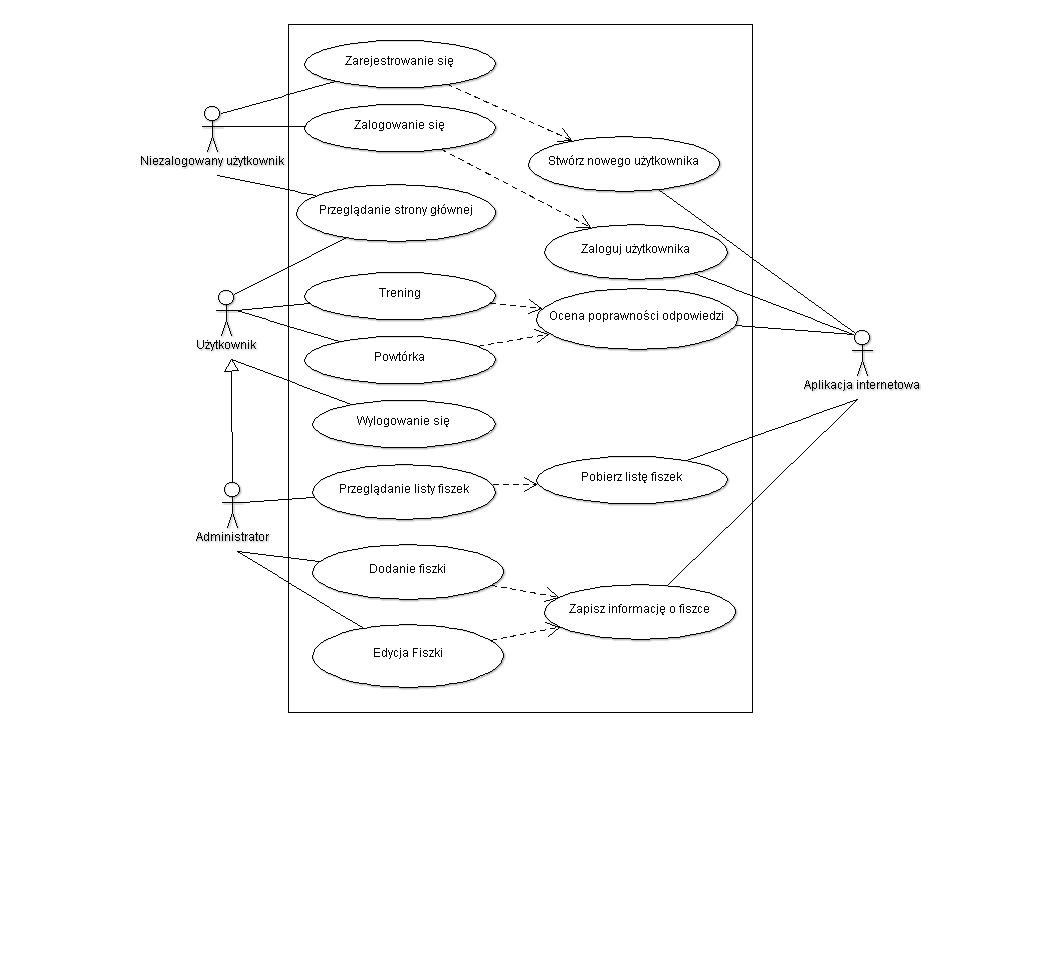
\includegraphics[width=\textwidth]{images/usecases.png}
	 \caption{Diagram przypadków użycia.}
\end{figure}


\section{Proces nauczania}

Proces nauczania jest podzielony na 2 etapy :
\begin{itemize}
	\item Trening
	\item Powtórkę
\end{itemize}

\subsection{Trening}

W trakcie treningu użytkownik po raz pierwszy może spotkać się z danym słowem występującym w procesie nauki. Celem tego etapu jest zaznajomienie użytkownika z nowym słowem, zanim zacznie go używać w ramach powtórki.
Trening korzysta z kolejki, wewnątrz której znajduje się maksymalnie 5 fiszek. Tak mała ilość ma na celu łatwiejsze przyswojenie nowego materiału.

W przypadku poprawnej odpowiedzi na pytanie fiszka jest usuwana z kolejki i dodawana do zapamiętanych fiszek, w przeciwnym wypadku przechodzi na koniec kolejki zwiększając ilość niepoprawnych odpowiedzi o 1.

\subsection{Powtórka}

W powtórce mogą wystąpić jedynie te fiszki, na które użytkownik odpowiedział poprawnie w trakcie treningu. Ten etap także składa się z kolejki, lecz jest ona maksymalnie 30 elementowa. 

W przypadku poprawnej odpowiedzi na pytanie fiszka jest usuwana z kolejki i obliczany dla nie jest jest nowy interwał oraz siła z jaką jest zapamiętana. W przeciwnym wypadku fiszka jest przesuwana w pewne miejsce kolejki obliczane na podstawie poprzednich niepoprawnych odpowiedzi na tą fiszkę w danej powtórce.

\subsubsection{Miejsce w kolejce}

Miejsce w którym fiszka znajduje się po niepoprawnej odpowiedzi jest obliczane tylko na podstawie ilości poprzednich niepoprawnych odpowiedzi i wygląda następująco:
\begin{minipage}
\begin{center}
\begin{tabular}{| l | l | l |}
\hline
Ilość złych odpowiedzi  & Minimalna pozycja w kolejce & Maksymalna pozycja w kolejce \\ \Xhline{3\arrayrulewidth}

0 & $\frac{1}{3}$ & $\frac{1}{2}$   \\ \hline
1 & $\frac{1}{4}$  & $\frac{1}{3}$   \\ \hline
2 lub więcej & $\frac{1}{5}$   & $\frac{1}{5}$   \\ \hline
\end{tabular}
\label{table:internals}
\end{center}
\end{minipage}

\begin{figure}[!b]
	\centering
	\includegraphics[width=\textwidth]{images/interval.png}
	 \caption{Przykład miejsc umieszczenie fiszki w kolejce w wypadku złej odpowiedzi. Zobrazowanie informacji zawartych w tabeli \ref{table:internals}}
\end{figure}


\todo[inline]{Przypis dokończ}

\subsection{Siła}

\section{Narzędzia administratorskie}

\section{Diagramy klas}


\begin{figure}[h]
	\centering
	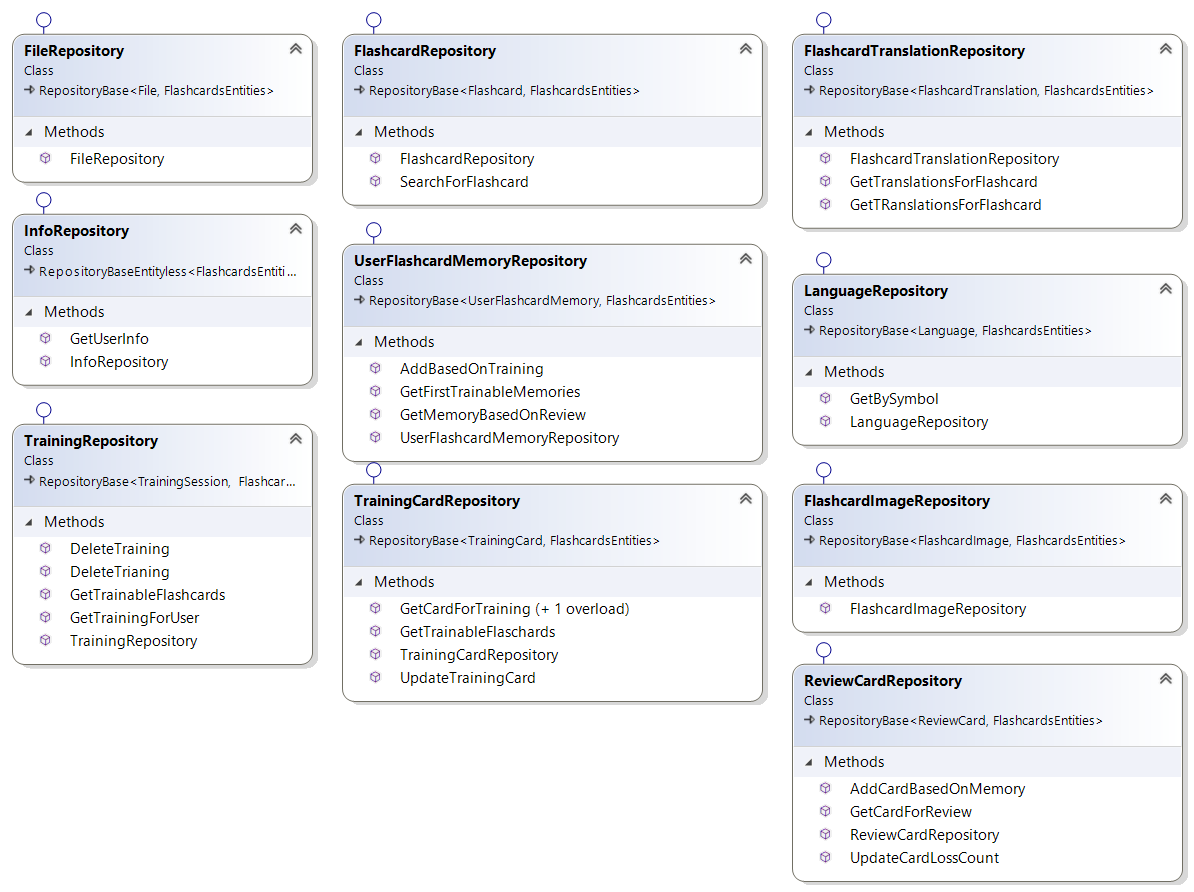
\includegraphics[width=\textwidth]{images/Repos.png}
	 \caption{Diagram klas wszystkich repozytoriów w projekcie wraz z jednostką pracy.}
\end{figure}


\begin{figure}
	\centering
	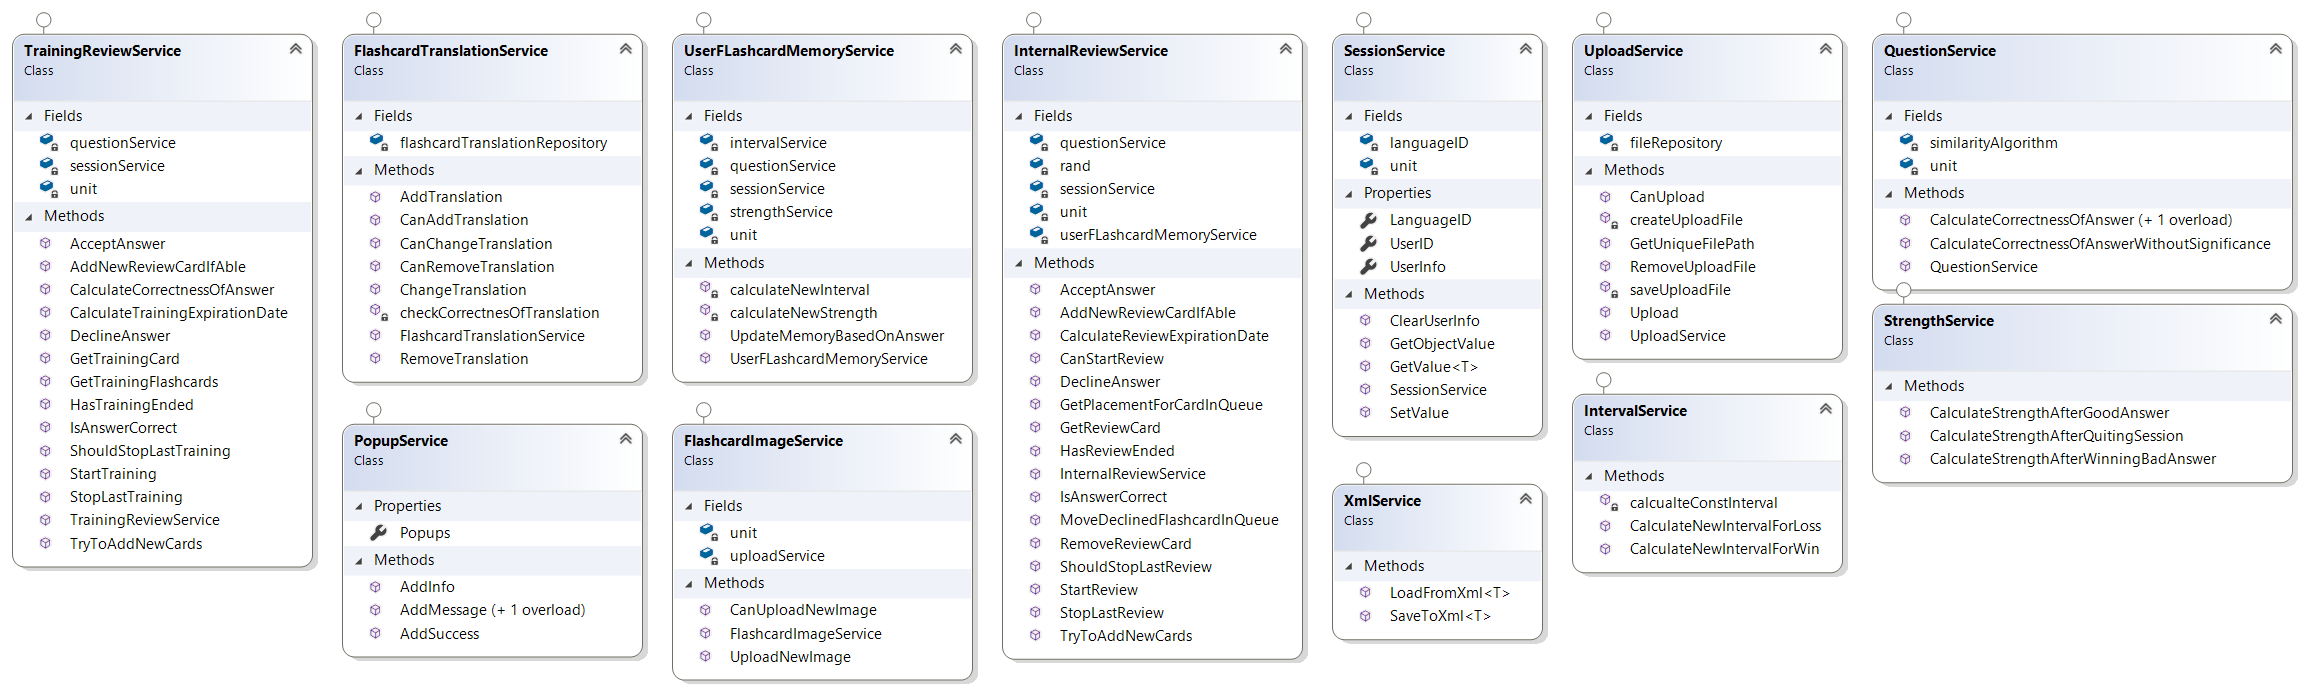
\includegraphics[width=\textwidth]{images/Serwisy.png}
	 \caption{Diagram klas wszystkich serwisów w projekcie}
\end{figure}


\begin{figure}
	\centering
	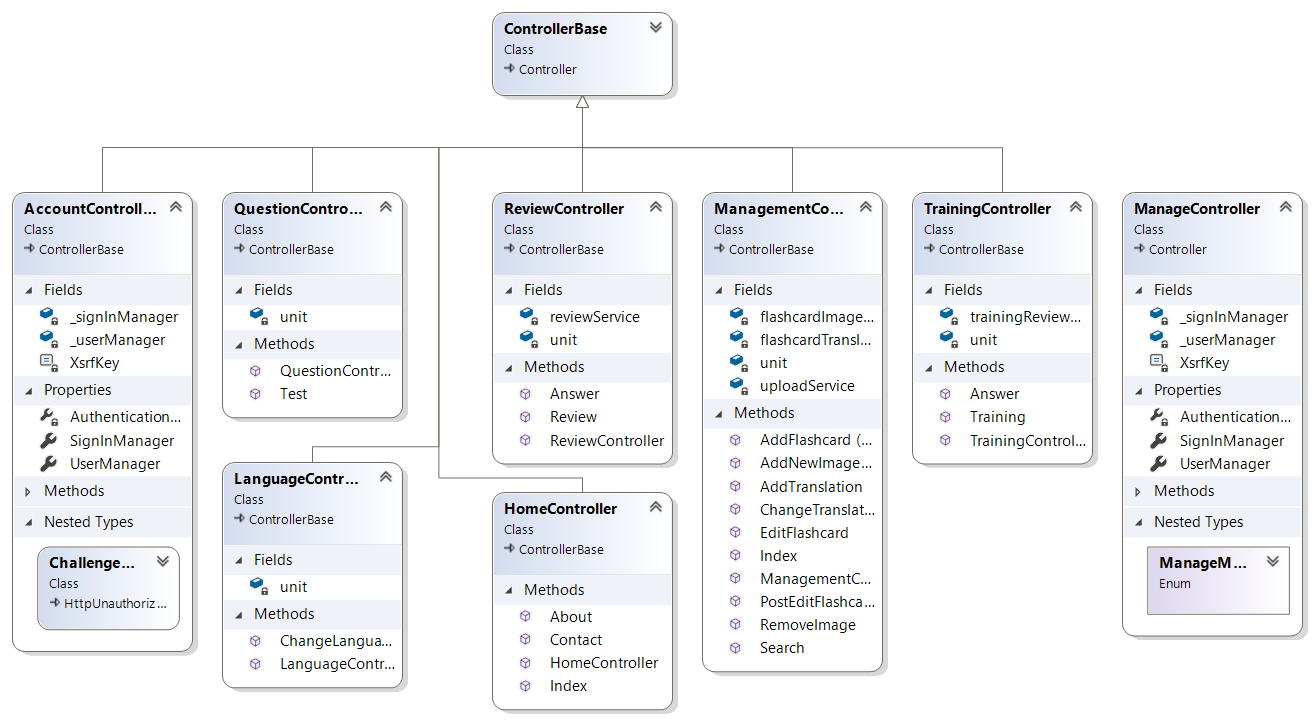
\includegraphics[width=\textwidth]{images/Controllers.png}
	 \caption{Diagram klas wszystkich kontrolerów w projekcie}
\end{figure}




\newpage
{\let\cleardoublepage\relax \chapter{Kwestie implementacyjne}}

\section{Struktura programu}

\section{Przechowywanie danych}

\section{Wyświetlanie stron}
